\section{球体}\label{sec:球体}

\keyindex{球}{sphere}{}是称为\keyindex{二次曲面}{quadrics}{}——
由$x,y$和$z$的二次多项式描述的通用类型曲面的一种特殊情况。
它是最简单的曲面类型,对光线追踪器很有用,是通用光线相交例程很好的起点。
pbrt支持六种二次曲面:球、\keyindex{圆锥体}{cone}{}、
\keyindex{圆盘}{disk}{}(圆锥的一种特例)、\keyindex{圆柱体}{cylinder}{}、
\keyindex{双曲线体}{hyperboloid}{}和\keyindex{抛物面}{paraboloid}{}。

许多曲面能以两种主要方式之一
描述:\keyindex{隐式形式}{implicit form}{}和\keyindex{参数形式}{parametric form}{}。
隐式函数将3D曲面描述为
\begin{align*}
    f(x,y,z)=0\, .
\end{align*}

所有满足该条件的点$(x,y,z)$的集合定义了该曲面。
对于位于原点的单位球体,熟悉的隐式函数是$x^2+y^2+z^2-1=0$。
只有距离原点一单位的点的集合才满足该约束,给出单位球的表面。

许多曲面也能用函数将2D点映射为曲面上的3D点来参数化地描述。
例如,半径为$r$的球体可以描述为2D球面坐标$(\theta,\varphi)$的函数,
其中$\theta$范围是从$0$到$\pi$,$\varphi$范围是从$0$到$2\pi$(\reffig{3.4}):
\begin{align*}
    x & =r\sin\theta\cos\varphi\, , \\
    y & =r\sin\theta\sin\varphi\, , \\
    z & =r\cos\theta\, .
\end{align*}
\begin{figure}[htbp]
    \centering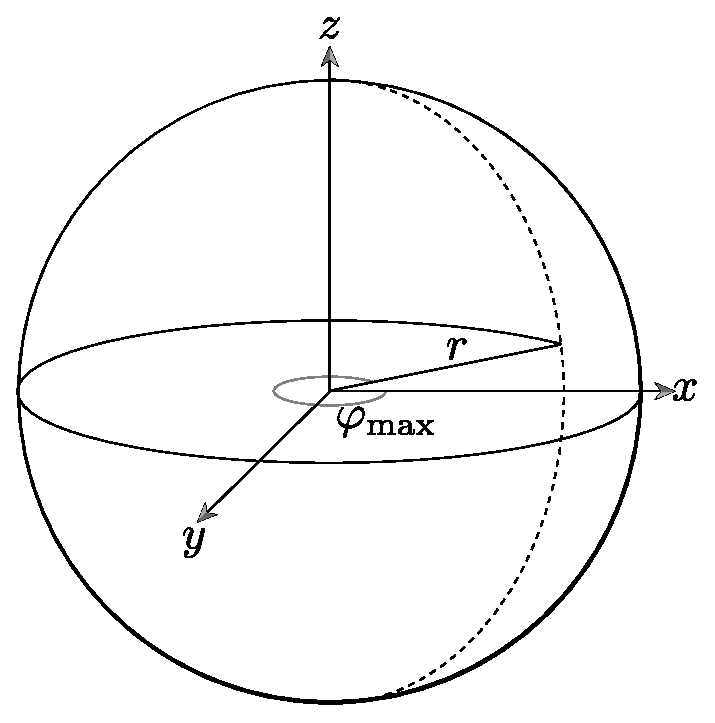
\includegraphics[width=0.5\linewidth]{chap03/Spheresetting.eps}
    \caption{球体形状基本设置。它半径为$r$,球心位于物体空间原点。
        部分球体可以通过指定$\varphi$的最大值描述。}
    \label{fig:3.4}
\end{figure}

我们可以用以下替换将该函数$f(\theta,\varphi)$转换为$[0,1]^2$上的函数$f(u,v)$并
稍微将其一般化以允许部分球体只扫过$\theta\in[\theta_{\min},\theta_{\max}]$和$\varphi\in[0,\varphi_{\max}]$:
\begin{align*}
    \varphi & =u\varphi_{\max}\, ,                              \\
    \theta  & =\theta_{\min}+v(\theta_{\max}-\theta_{\min})\, .
\end{align*}

该形式对纹理贴图特别有用,它能直接用来
将定义在$[0,1]^2$上的纹理映射到球上。
\reffig{3.5}展示了两个球的一张图像;一张网格图像用于展示$(u,v)$参数化。
\begin{figure}[htbp]
    \centering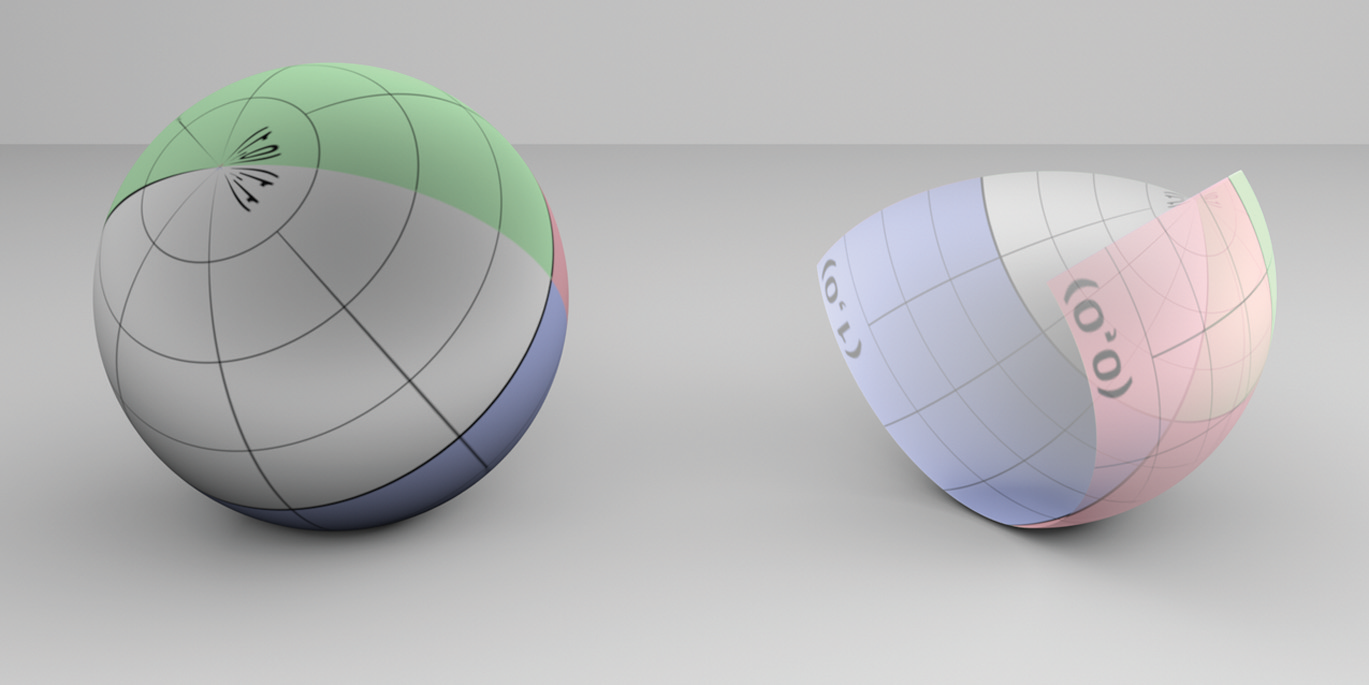
\includegraphics[width=\linewidth]{chap03/twospheres.png}
    \caption{两个球。左边是完整球,右边是部分球($z_{\max}<r$和$\varphi_{\max}<2\pi$)。
        注意纹理贴图用来展示形状$(u,v)$参数化;一极的\protect\keyindex{奇点}{singularity}{}在完整球中可见。}
    \label{fig:3.5}
\end{figure}

当我们描述球形状的实现时,我们将同时利用形状的隐式和参数化描述,
这取决于哪种方式能更自然地解决我们面临的特定问题。

类\refvar{Sphere}{}表示球心在物体空间原点的球体。
其实现在\href{https://github.com/mmp/pbrt-v3/tree/master/src/shapes/sphere.h}{\ttfamily shapes/sphere.h}
和\href{https://github.com/mmp/pbrt-v3/tree/master/src/shapes/sphere.cpp}{\ttfamily shapes/sphere.cpp}文件中。
\begin{lstlisting}
`\initcode{Sphere Declarations}{=}`
class `\initvar{Sphere}{}` : public `\refvar{Shape}{}` {
public:
    `\refcode{Sphere Public Methods}{}`
private:
    `\refcode{Sphere Private Data}{}`
};
\end{lstlisting}